\section{Semiconductor detectors \cite{semi}}
Semiconductors are solid states with periodic lattice structure and their important feature is the size of their band gap. While they are isolator at a temperature of absolute zero, their conductivity grows exponentially with the temperature. This is due to the thermal energy being able to excite a valence electron into the conduction band.
\subsection{Properties of semiconductors}
For intrinsic semiconductors the conductivity is only given by the electron moving into the conduction band and the reminding hole in the valence band. They are interpretated as positive charge carrier. Real crystals usually have imperfections due to chemical impurities or structural defects, which slightly changes the properties. \\
\begin{figure}
	\center
	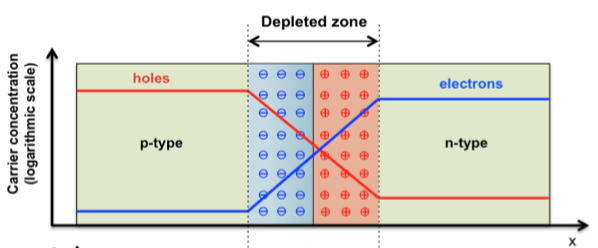
\includegraphics[width=0.6\textwidth]{graphics/pn.png}
	\caption{Diagram of the interference region of a p-n juntion. \cite{ali}}
	\label{fig:pn}
\end{figure}
Doping is a method where intentionally impurities are added to the lattice. This are usually atoms with an additional or one valence electron less to create n-doped (free electron) or p-doped (free hole) semiconductors. Adding a p- und n-doped Semiconductor together creates a p-n junction which is the base of all present semiconductor devices. Figure \ref{fig:pn} shows a schematic representation of a p-n junction. Due to the different carrier concentrations, they start drifting into eachother and recombine. This creates the depletion zone, which does not contain any free charge carrier. Applying an external voltage to the p-n junction in reverse biasing (anode to the n-side, cathode to the p-side) enlarges the width of the depletion zone, while applying the forward-biasing (anode to the p-side, cathode to the n-side) decreases its width. The reverse biasing ensures that the semiconductor detector behaves like a diode. In this condition a small current flows until a breakdown voltage is reached. The best condition to use a semicondutor devise as detector is with a high enough voltage so the depletion zone occupies the whole sensor. This condition is called fully depleted and there are no free charge carriers present. If a charged particle crosses the fully depleted sensor, it leaves an ionization track which can be measured with the electronics at the surface of the semicondutor. \\
The leakage current is main background for the signal collected with a semiconductor detector. Its main source is thermally generated electron-hole pairs in the depletion zone. To decrease this leakage current the sensors are usually cooled.\\
The semiconductors have severeal advantages compared to gas chambers due to their properties. They have good tracking properties in terms of time and spatial resolution. They also have a rapid charge-collection of $\sim\SI{10}{\nano\second}$ due to the higher density which makes them suitable for HEP experiment conditions. This also leads to a greater stopping power and allows to build thinner detectors. Another benefit is the ionization energy of just $\sim\SI{3}{\electronvolt}$ compared to $\sim\SI{30}{\electronvolt}$ for gas-based detectors. This leads to a better signal and energy resolution. The only significant downside is that they suffer a significant degradation from radiation-induced damage during their lifetime. The two mainly used materials are Silicon and Germanium. Germanium has a higher atomic number and therefore is better for $\gamma$-ray detection. But due to the small band gap energy it needs cooling, while Silicon can be operated at room temperature. It is also cheaper and therefore the mainly used material at HEP detectors e.g. at the large hadron collider (LHC) experiments at CERN.
\subsection{Historical development of semiconductor detectors}
In 1949 K. G. McKay published a paper about a Germanium point-contact diode, which was the first semiconductor detector. In the 1960s monocrystalline siicone became aviable. In the 1970s Boyle and Smith published their concept for Charge-Couple Devices (CCD), which was later rewarded with the Nobel prize. J. Kemmer finally introduced the planar technology to build diodes and transitors in 1979. This was the revolution in silicon detectors leading to the advanced forms of strip and pixel sensors. The HEP experiments NA11-NA32 were then the first experiments using silicon microstrip sensor to c´study charm physics. In 1994 DELPHI installed the first silicon vertex detector. This principles are still being used at current HEP experiments with upgraded technologies.
\subsection{Silicon detector technologies}
\textit{Silicon Drift Detectors} use the principle of sidewards depletion, where the electric field is parallel to the surface of the silicon waver. Hence the position is measured trough the drift time. There are also able to measure the energy of the ionising radiation. Different shapes of the electrodes allow flexible configuration e.g. matrix drift devices that allow to perform a 2D position measurement.\\
\textit{Charged Coupled Devices} (CCD) are devices for the movement of electric charges. Together with silicon drift chambers they are called fully depleted pn CCDs and are able to detected particles and especially x-rays. The advantages are an enhanded sensitivity, an uniform responce and high speed of operation.\\
\textit{Strip Detectors} usually have a n-type silicon bulk, a $\text{n}^+$-type backplane, where the positive bias voltage will be applied and $\text{p}^+$-type strip implants. The higher doping leads to a faster collection of the signal. The trips are covered with a silicon dioxide layer to prevent current directly draining into the delicate readout electronics. The thickness of the whole sensor is usually \SI{300}{\micro\meter}. Future silicon sensors will have p-type silicon bulk and $\text{n}^+$-type strips. One of the advantage of this configuration is that the sensors can be operated even if they are not fully depleted. \textit{Double Sided} Strip Detectors have instead of the $\text{n}^+$-type backplane strips, that are turned \SI{90}{\degree} compared to the other strips. The allows a 2D information, but they are more complicated to produce since both sides need to be processed.\\
\textit{Pixel Detectors} are the most advantageous ones, since they provide 3D informations. They are build out of a 2D matrix of diodes, where each pixel gets its own readout chip. The common technology is the hybrid design, where pixel and readout electronics are produced seperatly and bump bonded together. The disadvantage are that Pixel detectors are expensive and produce a large data volumen. For this reason there are usually just used in the most inner parts of detectors. 
